\documentclass[11pt, oneside]{article} 	% use "amsart" instead of "article" for AMSLaTeX format
\usepackage{geometry} 		% See geometry.pdf to learn the layout options. There are lots.
\geometry{letterpaper}  		% ... or a4paper or a5paper or ... 
\usepackage[parfill]{parskip} 		% Activate to begin paragraphs with an empty line rather than an indent
\usepackage{graphicx}				% Use pdf, png, jpg, or eps§ with pdflatex; use eps in DVI mode
								% TeX will automatically convert eps --> pdf in pdflatex		
\usepackage{amssymb}
\usepackage{amsmath}
\usepackage{authblk}
\usepackage[
backend=biber,
style=alphabetic,
]{biblatex}
\usepackage{graphicx}
\graphicspath{ {./images/} }
\usepackage{verbatim}
\usepackage{tikz} 
\usepackage{subcaption}
\captionsetup{compatibility=false}



\usepackage{syntonly}

% \syntaxonly \langle -- use this for checking syntax only
% \mbox {text} - keep together
% \fbox {text} - keep together and draw around

%\pagestyle{plain|headings|empty} % header and footer p.27
%SetFonts
%\include{filename}, \includeonly{filename1, filename2} , \input[fiename}

%SetFonts% 


\title{Polynomial Uniqueness by way of Tournament Graphs}
\author{Dave Fetterman}
\affil{Obviously Unemployed}
\date{2/10/23}
\begin{document}
\maketitle

\begin{abstract}

In 2D space, two points $(x_1, y_1), (x_2, y_2), x_1 \neq x_2$ define a line, a polynomial of degree 1.  Three distinct points $(x_1, y_1), (x_2, y_2), (x_3, y_3) x_1 \neq x_2 \neq x_3 \neq x_1$ define a parabola, a polynomial of degree 2.  In general, for finite univariate polynomials of nonnegative, whole degree, $n+1$ such points uniquely specify a polynomial of degree $n$.  Why?
\\

This is not a new result. This is a paper is simply a thoroughly awkward trip through a few mathematical domains to arrive at a well known destination. Helicopters and cars both have their uses. But you wouldn't build a car by turning a helicopter on its side and adding wheels.  
\\

Metaphorically, I do, so you don't have to.

\end{abstract}

\section{Setup}

If we have points $f(x_1) = y_1, f(x_2) = y_2, \ldots f(x_{n+1}) = y_{n+1}$, how can we determine the coefficients $a_i$ of the polynomial $f(x) = a_0x^0 + a_1x^1 + \ldots + a_nx^n$?

This matrix $X$, known as a Vandermonde matrix\cite{1}, models this set of equations as $X \cdot \vec{a} = \vec{y}$:

 $\begin{bmatrix}
1 & x_0 & x_0^2 & \ldots & x_0^{n} \\
1 & x_1 & x_1^2 & \ldots & x_1^{n} \\
\vdots & & & & \vdots  \\
1 & x_{n+1} & x_{n+1}^2 & \ldots & x_{n+1}^{n} \\
\end{bmatrix}
\cdot 
\begin{bmatrix}
a_0 \\
a_1 \\
\vdots \\
a_n \\
\end{bmatrix}
=
\begin{bmatrix}
y_1 \\
y_2 \\
\vdots \\
y_{n+1} \\
\end{bmatrix}
$
Therefore, we can find our unique coefficient vector $A$ if and only if we can solve $X \cdot \vec{a} = \vec{y}$, or $\vec{a} = X^{-1} \vec{y}$.  This has a unique solution if and only if $\det(X) \neq 0$.  The rest of this paper tries to find this determinant through all the wrong ways.

\section{Finding the Vandermonde determinant}

It should be noted that there are other, clearer methods of finding this determinant\cite{1} either starting with polynomial unqiueness (basically, going the ``other'' direction), abstract algebra, direct linear algebra, vector maps, and likely others.  These, however, were not the ones I stumbled on.

First, we know that if any $x_i = x_j$ for distinct $i, j$, we have no solution, and a zero determinant. If $f(x_i) = f(x_j), x_i = x_j$, then we are simply underdetermined (not enough points for a unique polynomial).   If $f(x_i) = f(x_j), x_i \neq x_j$, then we have a impossible vertical section of our graph.  Otherwise, we are in good shape.  
\\

This suggests that every pair $(x_i, x_j), i < j$ corresponds to a factor  $(x_j - x_i)$ in the determinant, and that the determinant is then some multiple of $D = \prod_{0 \leq i < j \leq n}(x_j-x_i)$.

Taking $n=2$ as a base case ($n=1$ produces a constant $f(x)$), we see that 
 $\det\begin{bmatrix}
1 & x_0  \\
1 & x_1  \\
\end{bmatrix} = (x_1 - x_0)$, suggesting our determinant is exactly $D$.

The rest of the paper will be handling the inductive step in the most roundabout way possible.

\section{Prove : VanDerMonde matrix determinant is prod $(x_i - x_j), 1 <= i < j <= n$}
 This is the determinant of the van der modne matrix
\subsection{Base cane: n = 2}
\subsection{Inductive case} This equals$ x^n$ (product without x), +$ y^n $(product without y)...
\begin{comment}
- Represent as a graph tournament, n nodes, (n choose 2) edges.  There are 2^(n choose 2) possibilities.
- Each term (+/-) x_0^a_0*x_1^a_1...*x_n^a_n, where sum a_i = (n choose 2), represents one possible tournament on a directed complete graph of size n
- If there are no cycles in a given tournamnet
  - then it's of the form b^n c^n-1 ... x^1 y^0 for some b,c,...y in x_i.
- If there are ctycles in a tournament
  - Any even cycle implies an odd cycle (quick proof)
  - Therfore there's an odd cycle
  - Reversing an odd cycle produces a different graph with an odd cycle and flipped sign.
- For a tournament config that is NOT a topo sort (has a cycle)
  - There are as many positivies as negatives (PROVE?)
  - So the terms cancel out
  - Therefore everything is of the form b^n c^n-1 ... x^1 y^0
  - So big product up to n is x^n(prodcut without x) + y^n(product without y..).
*** This is zero if and only if x_i = x_j for some
*** Therefore, only one solution for n distinct points on a polynomial of size n.

\end{comment}

\section{Pieceyard}

% Graph drawing reference: https://www.baeldung.com/cs/latex-drawing-graphs

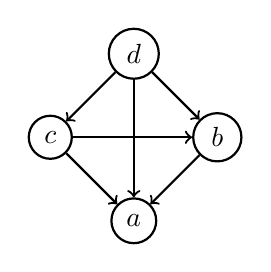
\begin{tikzpicture}[node distance={15mm}, thick, main/.style = {draw, circle}] 
\node[main] (1) {$a$}; 
\node[main] (2) [above right of=1] {$b$}; 
\node[main] (3) [above left of=1] {$c$}; 
\node[main] (4) [above right of=3] {$d$}; 
\draw[->] (4) -- (3); 
\draw[->] (4) -- (2); 
\draw[->] (4) -- (1); 
\draw[->] (3) -- (2); 
\draw[->] (3) -- (1);
\draw[->] (2) -- (1);
\end{tikzpicture}

The sorted tournament $d^3c^2b^1a^0$

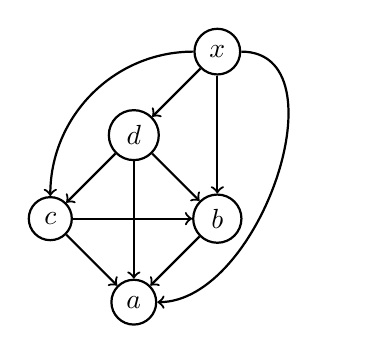
\begin{tikzpicture}[node distance={15mm}, thick, main/.style = {draw, circle}] 
\node[main] (1) {$a$}; 
\node[main] (2) [above right of=1] {$b$}; 
\node[main] (3) [above left of=1] {$c$}; 
\node[main] (4) [above right of=3] {$d$}; 
\node[main] (5) [above right of=4] {$x$}; 
\draw[->] (5) -- (4);
\draw[->] (5) to [out=180, in=90, looseness=1] (3); 
\draw[->] (5) -- (2);
\draw[->] (5) to [out=0, in=0, looseness=1] (1); 
\draw[->] (4) -- (3); 
\draw[->] (4) -- (2); 
\draw[->] (4) -- (1); 
\draw[->] (3) -- (2); 
\draw[->] (3) -- (1);
\draw[->] (2) -- (1);
\end{tikzpicture}

The sorted tournament $x^4d^3c^2b^1a^0$



\begin{figure}
\centering
\begin{subfigure}{.5\textwidth}
  \centering
  
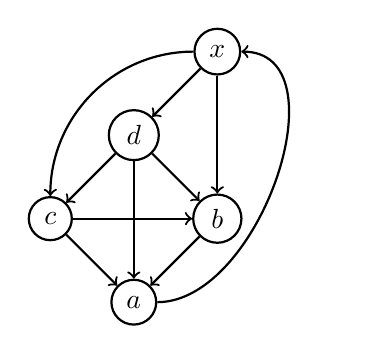
\begin{tikzpicture}[node distance={15mm}, thick, main/.style = {draw, circle}] 
\node[main] (1) {$a$}; 
\node[main] (2) [above right of=1] {$b$}; 
\node[main] (3) [above left of=1] {$c$}; 
\node[main] (4) [above right of=3] {$d$}; 
\node[main] (5) [above right of=4] {$x$}; 
\draw[->] (5) -- (4);
\draw[->] (5) to [out=180, in=90, looseness=1] (3); 
\draw[->] (5) -- (2);
\draw[->] (1) to [out=0, in=0, looseness=1] (5);
\draw[->] (4) -- (3); 
\draw[->] (4) -- (2); 
\draw[->] (4) -- (1); 
\draw[->] (3) -- (2); 
\draw[->] (3) -- (1);
\draw[->] (2) -- (1);
\end{tikzpicture}
  \caption{$-x^3a \cdot d^3c^2b^1a^0$, with cycle $(x b a)$}
  \label{fig:sub1}
\end{subfigure}%
\begin{subfigure}{.5\textwidth}
  \centering
  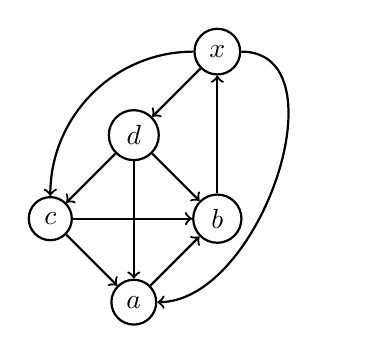
\begin{tikzpicture}[node distance={15mm}, thick, main/.style = {draw, circle}] 
\node[main] (1) {$a$}; 
\node[main] (2) [above right of=1] {$b$}; 
\node[main] (3) [above left of=1] {$c$}; 
\node[main] (4) [above right of=3] {$d$}; 
\node[main] (5) [above right of=4] {$x$}; 
\draw[->] (5) -- (4);
\draw[->] (5) to [out=180, in=90, looseness=1] (3); 
\draw[<-] (5) -- (2);
\draw[->] (5) to [out=0, in=0, looseness=1] (1);
\draw[->] (4) -- (3); 
\draw[->] (4) -- (2); 
\draw[->] (4) -- (1); 
\draw[->] (3) -- (2); 
\draw[->] (3) -- (1);
\draw[<-] (2) -- (1);
\end{tikzpicture}

  \caption{$-x^3b \cdot -d^3c^2a^1b^0$, with cycle $(x a b)$}
  \label{fig:sub2}
\end{subfigure}
\caption{Terms in expanded $\prod (x_j - x_i)$ are inverses with inverted 3-cycles }
\label{fig:test}
\end{figure}







Factors of $(x-a)(x-b)(x-c)(x-d)$ multiplied by $\sigma = d^3c^2b^1a^0$

\begin{center}
\begin{tabular}{||c c c c c||} 
 \hline
 Factor & Product & Matching Factor & Matching $\sigma$ & Critical pair \\ [0.5ex] 
 \hline\hline
 $x^4$ & $x^4d^3c^2b^1a^0$ & none & none & none \\ 
 \hline
 $-x^3a$ & $-x^3d^3c^2b^1a^1$ & $-x^3b$ & $-d^3c^2a^1b^0$ & $ba$ \\ 
 \hline
 $-x^3b$ & $-x^3d^3c^2b^2a^0$ & $-x^3c$ & $-d^3b^2c^1a^0$ & $cb$ \\ 
 \hline
 $-x^3c$ & $-x^3d^3c^3b^1a^0$ & $-x^3d$ & $-c^3d^2b^1a^0$ & $dc$ \\ 
 \hline
 $-x^3d$ & $-x^3d^4c^2b^1a^0$ & none & none & none \\ 
 \hline
 $x^2ba$ & $x^2d^3c^2b^2a^1$ & $x^2ca $& $-d^3b^2c^1a^0$ &  $cb$ \\ 
  \hline
 $x^2ca$ & $x^2d^3c^3b^1a^1$ & $x^2da $& $-c^3d^2b^1a^0$ &  $dc$ \\ 
 \hline
 $x^2da$ & $x^2d^4c^2b^1a^1$ & $x^2db $& $-d^3c^2a^1b^0$ &  $ba$ \\ 

 \hline
 $x^2cb$ & $x^2d^3c^3b^2a^0$ & $x^2db $& $-c^3d^2b^1a^0$ &  $dc$ \\ 
 \hline
 $x^2db$ & $x^2d^4c^2b^2a^0$ & $x^2dc $& $-d^3b^2c^1a^0$ &  $dc$ \\ 
 
 
\hline
 $x^2dc$ & $x^2d^4c^3b^1a^0$ & none & none &  none \\ 
 
 \hline
 $-xcba$ & $-xd^3c^3b^2a^1$ & $-xdba $& $-c^3d^2b^1a^0$ &  $dc$ \\ 

 \hline
 $-xdba$ & $-xd^4c^2b^2a^1$ & $-xcba $& $-d^3b^2c^1a^0$ &  $cb$ \\ 

 \hline
 $-xdca$ & $-xd^4c^3b^1a^1$ & $-xdcb $& $-d^3c^2a^1b^0$ &  $ba$ \\ 

 \hline
 $-xdcb$ & $-xd^4c^3b^2a^0$ & none & none &  none \\ 
 
 
 \hline
 $dcba$ & $ d^4c^3b^2a^1 $ & none & none &  none \\ 
 
 \hline
\end{tabular}
\end{center}


\section{TODO}
\subsection{TODO}

\begin{thebibliography}{9}
\bibitem{1}
Wikipedia: \url{https://en.wikipedia.org/wiki/Vandermonde_matrix}
\end{thebibliography}


\end{document}

